\section{Exploring the Parameter Space}
\label{ch:HourglassParameterSpace}

\subsection{Hourglass Parameters}
\begin{frame}{Exploring the Simulation Parameter Space}
In order to tune the Hourglass Simulation, I identified how various beam
parameters affected the final z-vertex profile.
\begin{columns}[T] % contents are top vertically aligned
\begin{column}[T]{5cm} % each column can also be its own environment
\begin{itemize}
\item Stretching/Squeezing of distribution
\item Asymmetry in peak heights
\item Individual Peak Widths
\item Peak Separation
\item Peak Scaling
\end{itemize}
\end{column}
\begin{column}[T]{5cm} % alternative top-align that's better for graphics
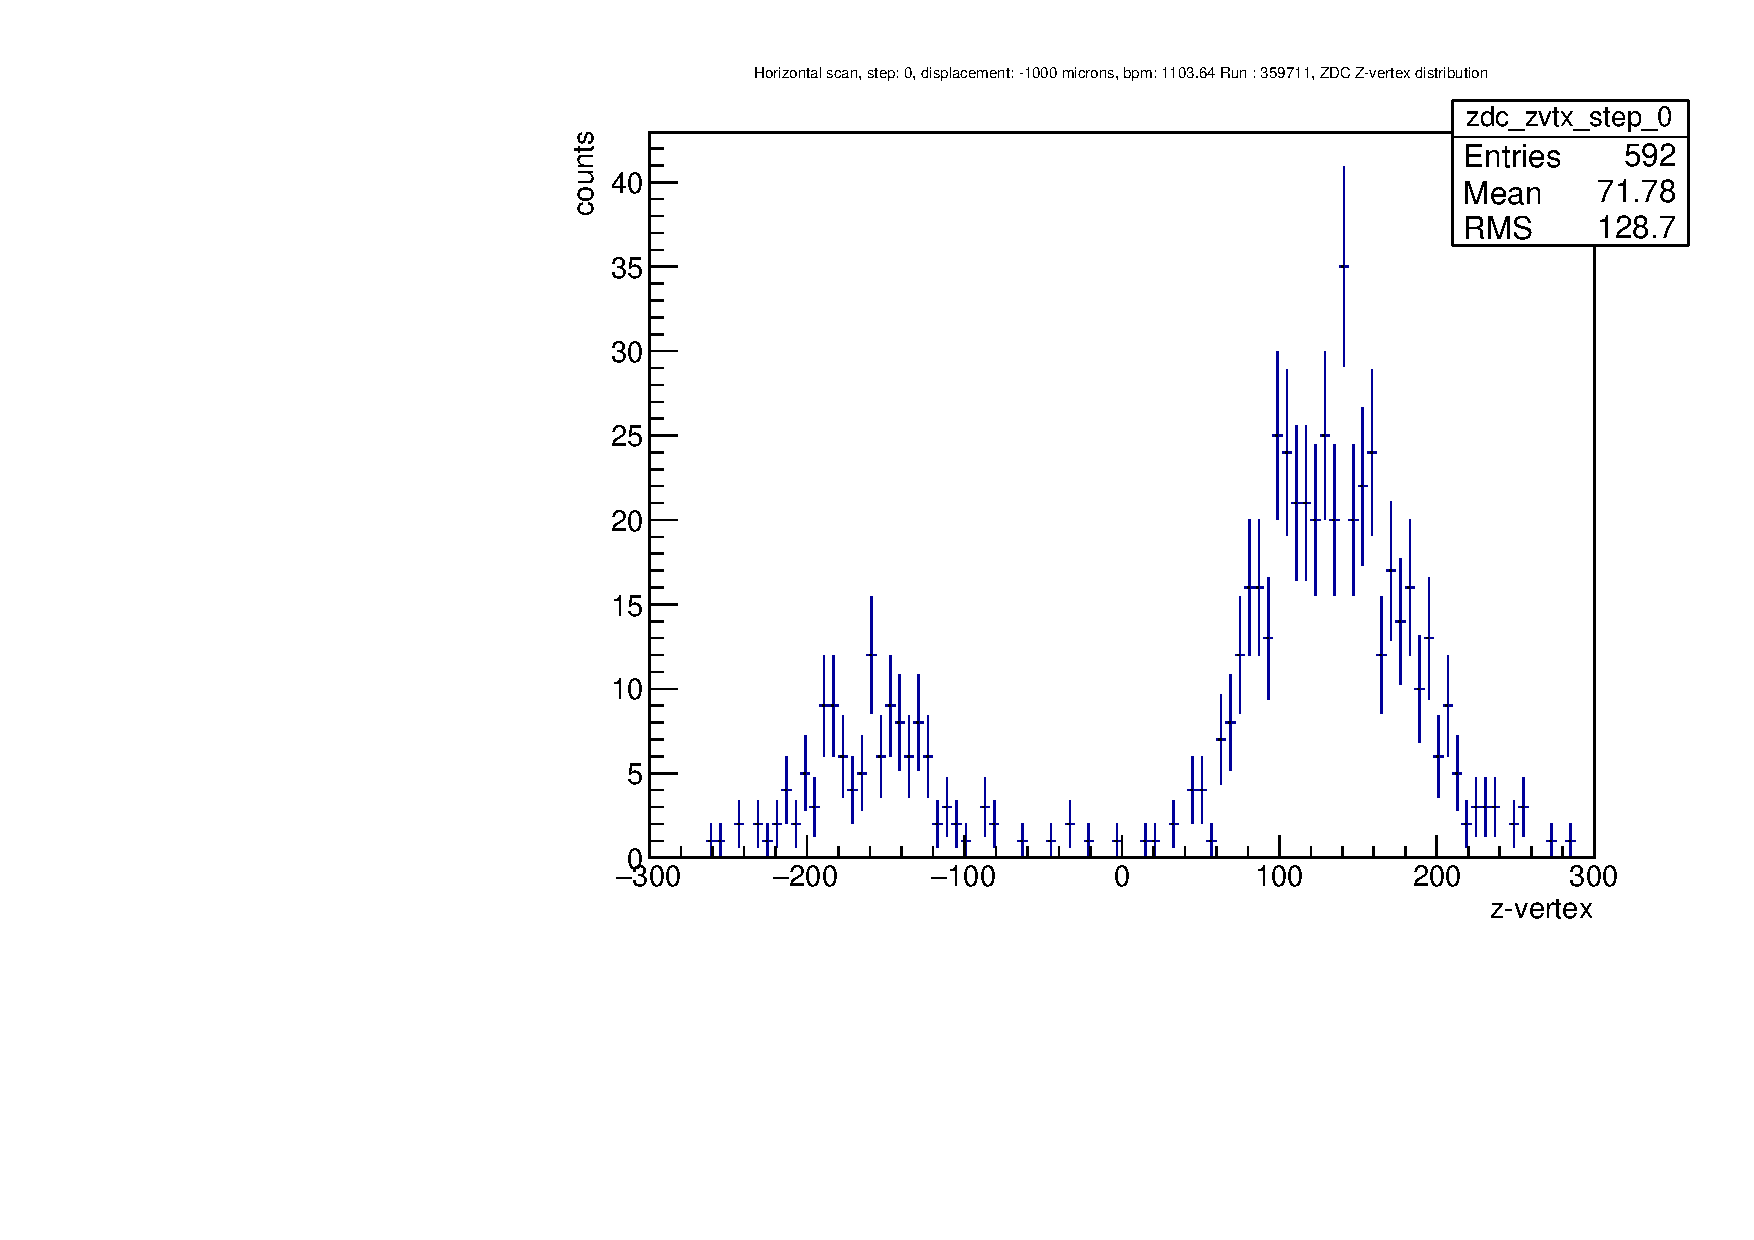
\includegraphics[width=\textwidth,height=\textheight,keepaspectratio]{../HourglassParameterSpace/figs/zvertex_profile_hscan_pos_1000_359711.pdf}
\end{column}
\end{columns}
\vspace{\baselineskip}
\textbf{Shown:} the zdc z-vertex histogram profile for -1000 micron beam
separation, $200 GeV$, run 359711. Characteristic hourglass effect (peak
separation) and crossing angle effect (peak asymmetry).
\end{frame}

\begin{frame}{Hourglass Parameters - \textcolor{red}{\textbf{Simulation}} and
	\textcolor{blue}{\textbf{Data}}}
\begin{center}
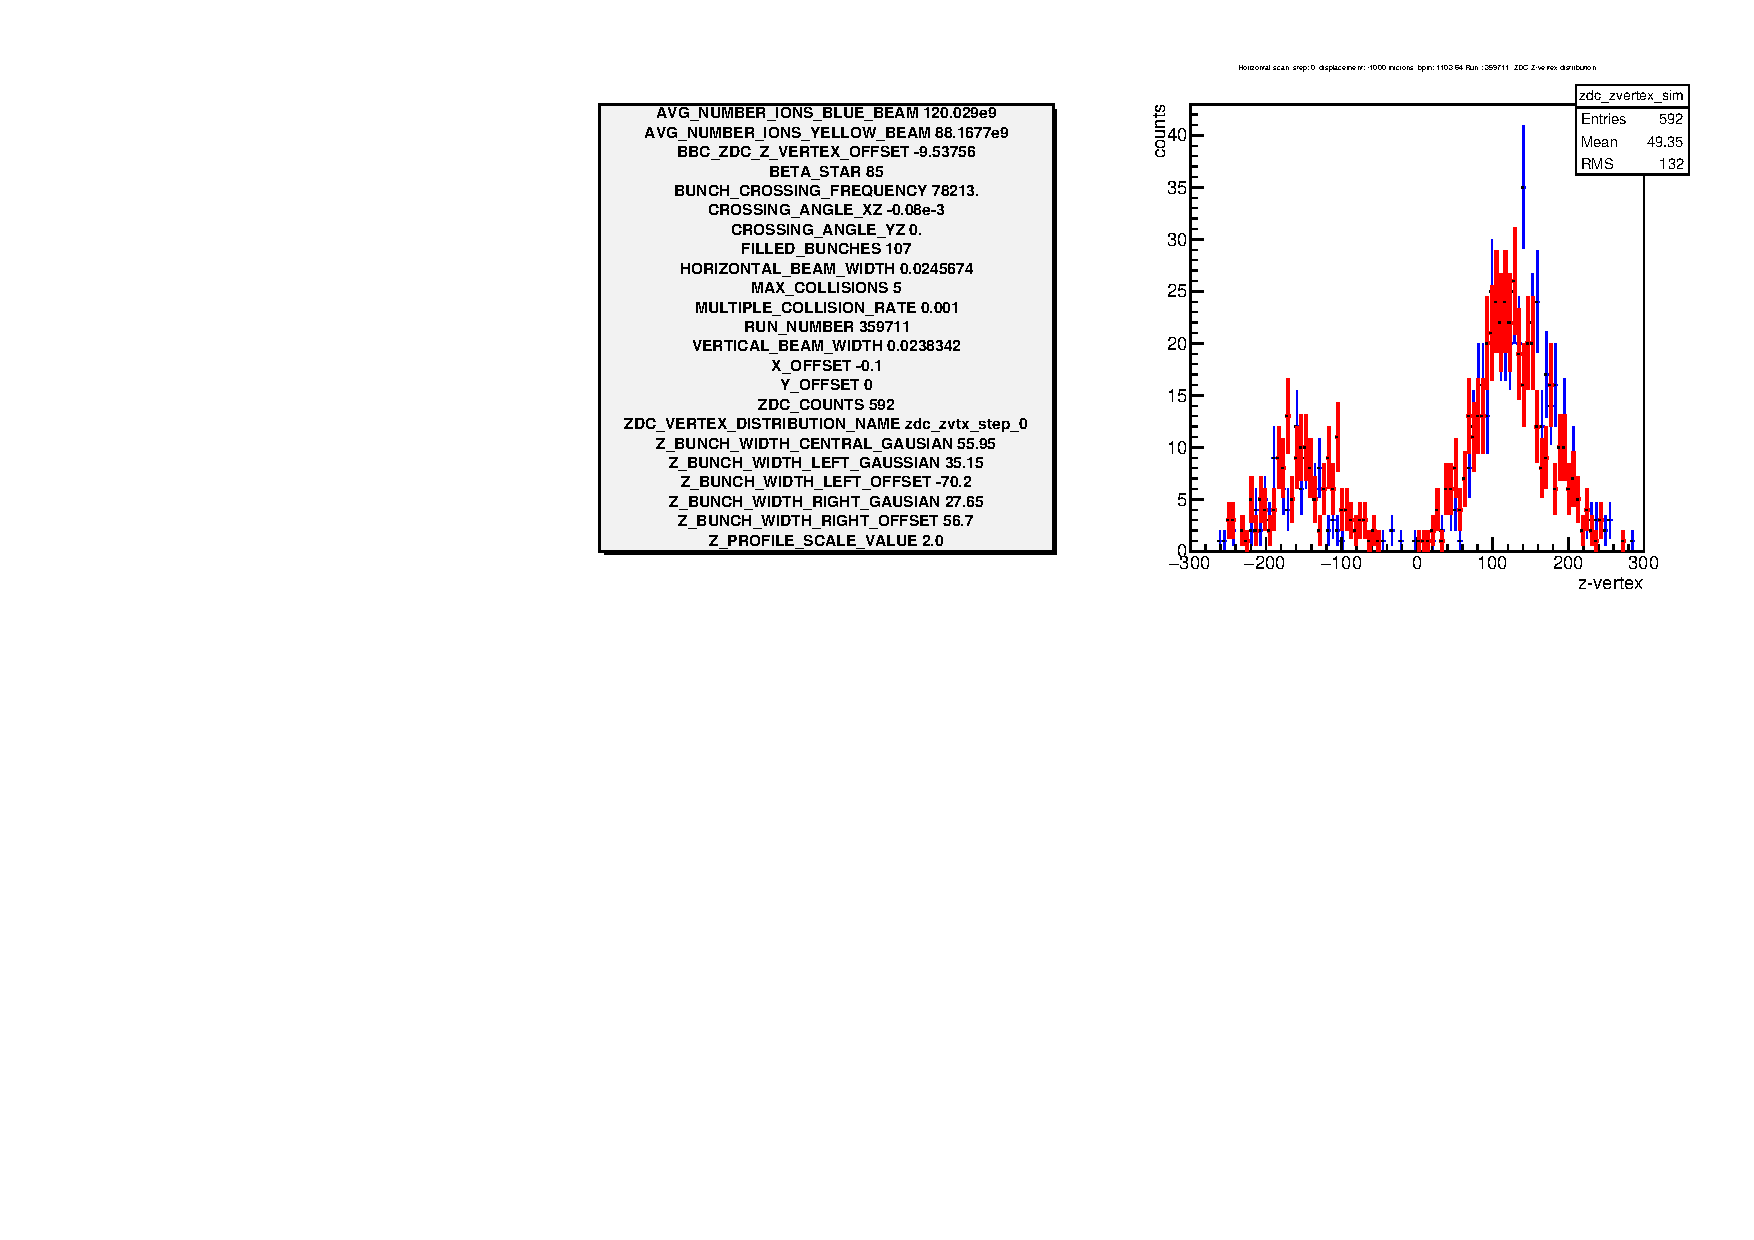
\includegraphics[scale=0.5]{../HourglassParameterSpace/figs/zvertex_compare_hscan_pos_1000_359711.pdf}
\end{center}

Here, we manually scale the simulation parameters to a achieve a reasonable
match for a scan step, -1000 microns (x), for 359711.

\vspace{\baselineskip}

Note that we use a general model for the z-profile (triple Gaussian, more on
this later), and achieve good matching through scaling this profile.
\end{frame}

\begin{frame}{Hourglass Parameters}

Starting from a reasonably matched spectra, we can now explore how modifying the
various parameters affect the output profile. 

\vspace{\baselineskip}

Smaller end of parameter range is shown in \textcolor{green}{\textbf{green}}
while larger end of parameter range is shown in \textcolor{pink}{\textbf{pink}}
\end{frame}

\begin{frame}{Large and Small $\beta^*$}
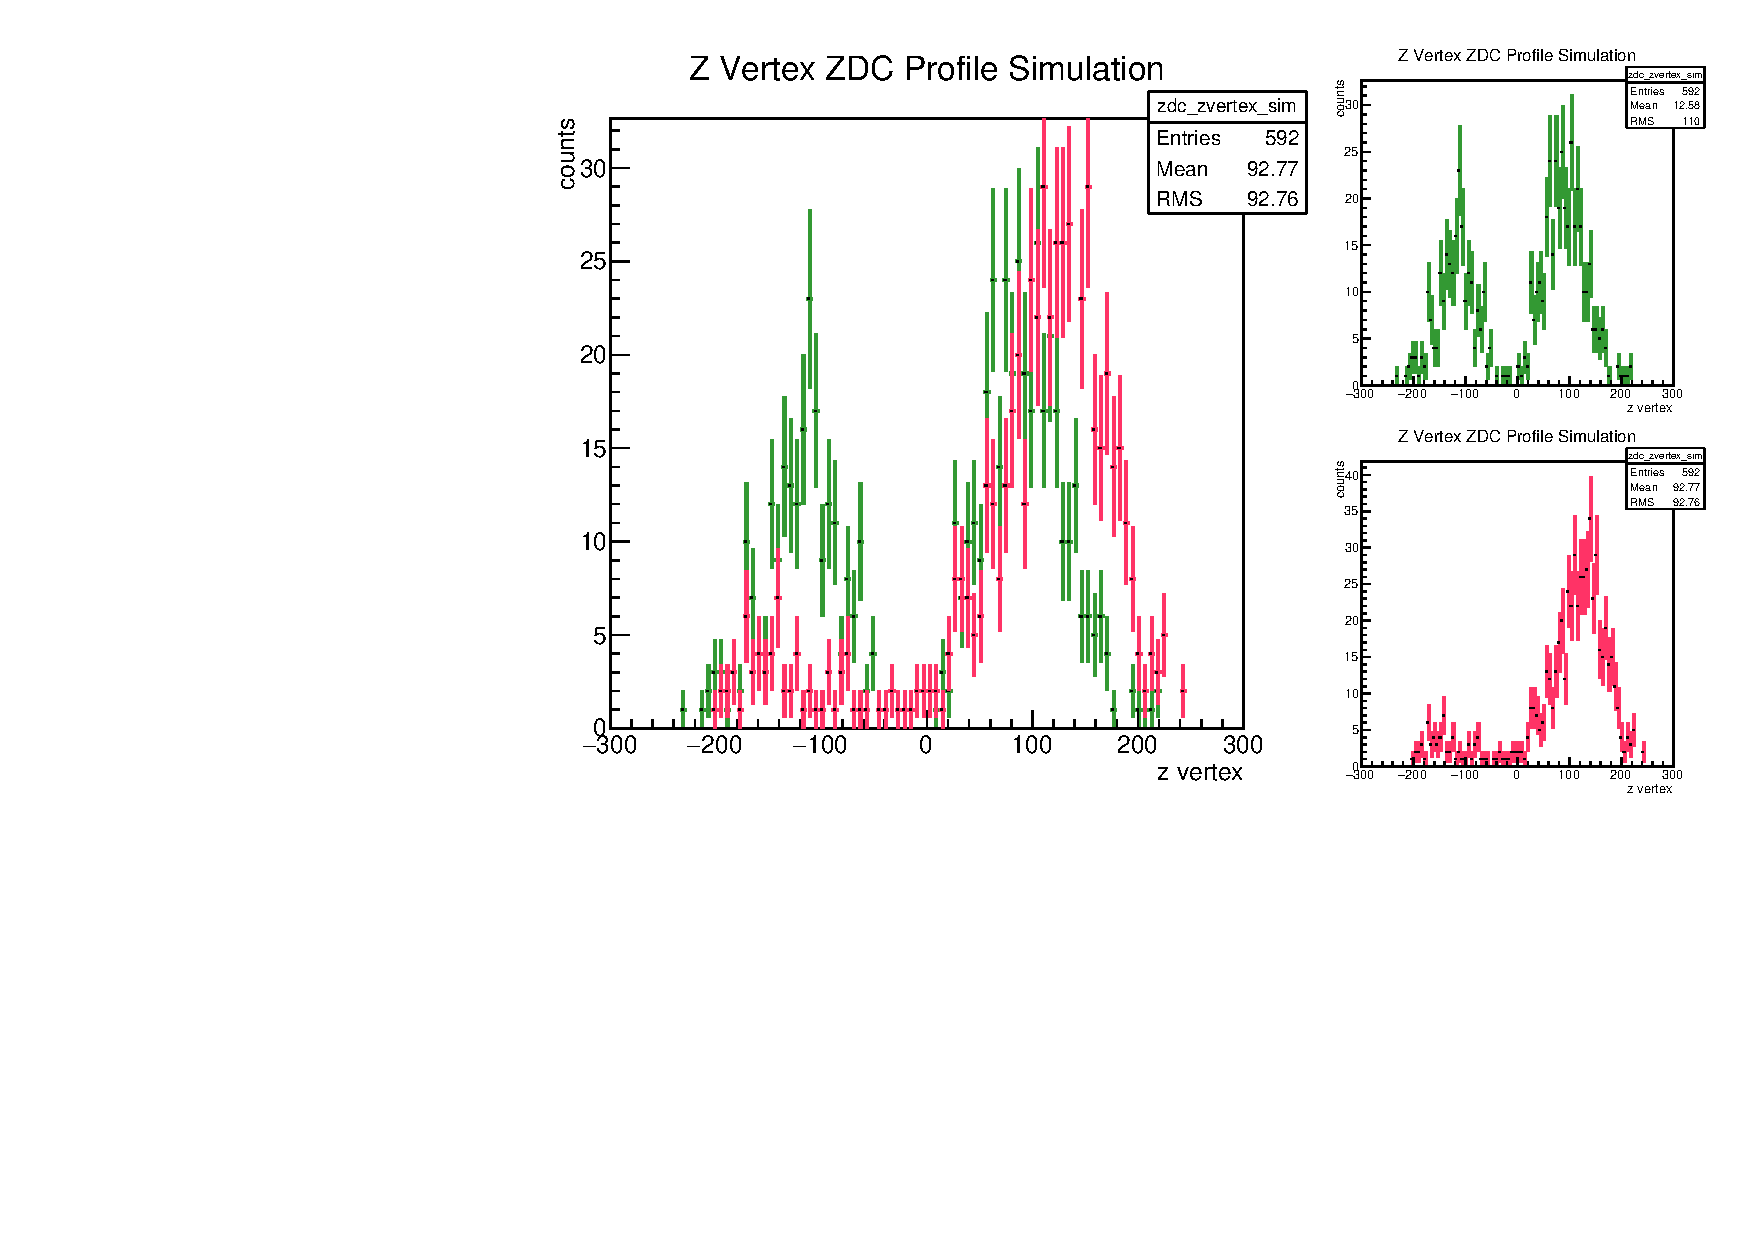
\includegraphics[width=\linewidth,height=\textheight,keepaspectratio]{../HourglassParameterSpace/figs/beta_star.pdf}
\end{frame}

\begin{frame}{Large and Small $\sigma_{x}$}
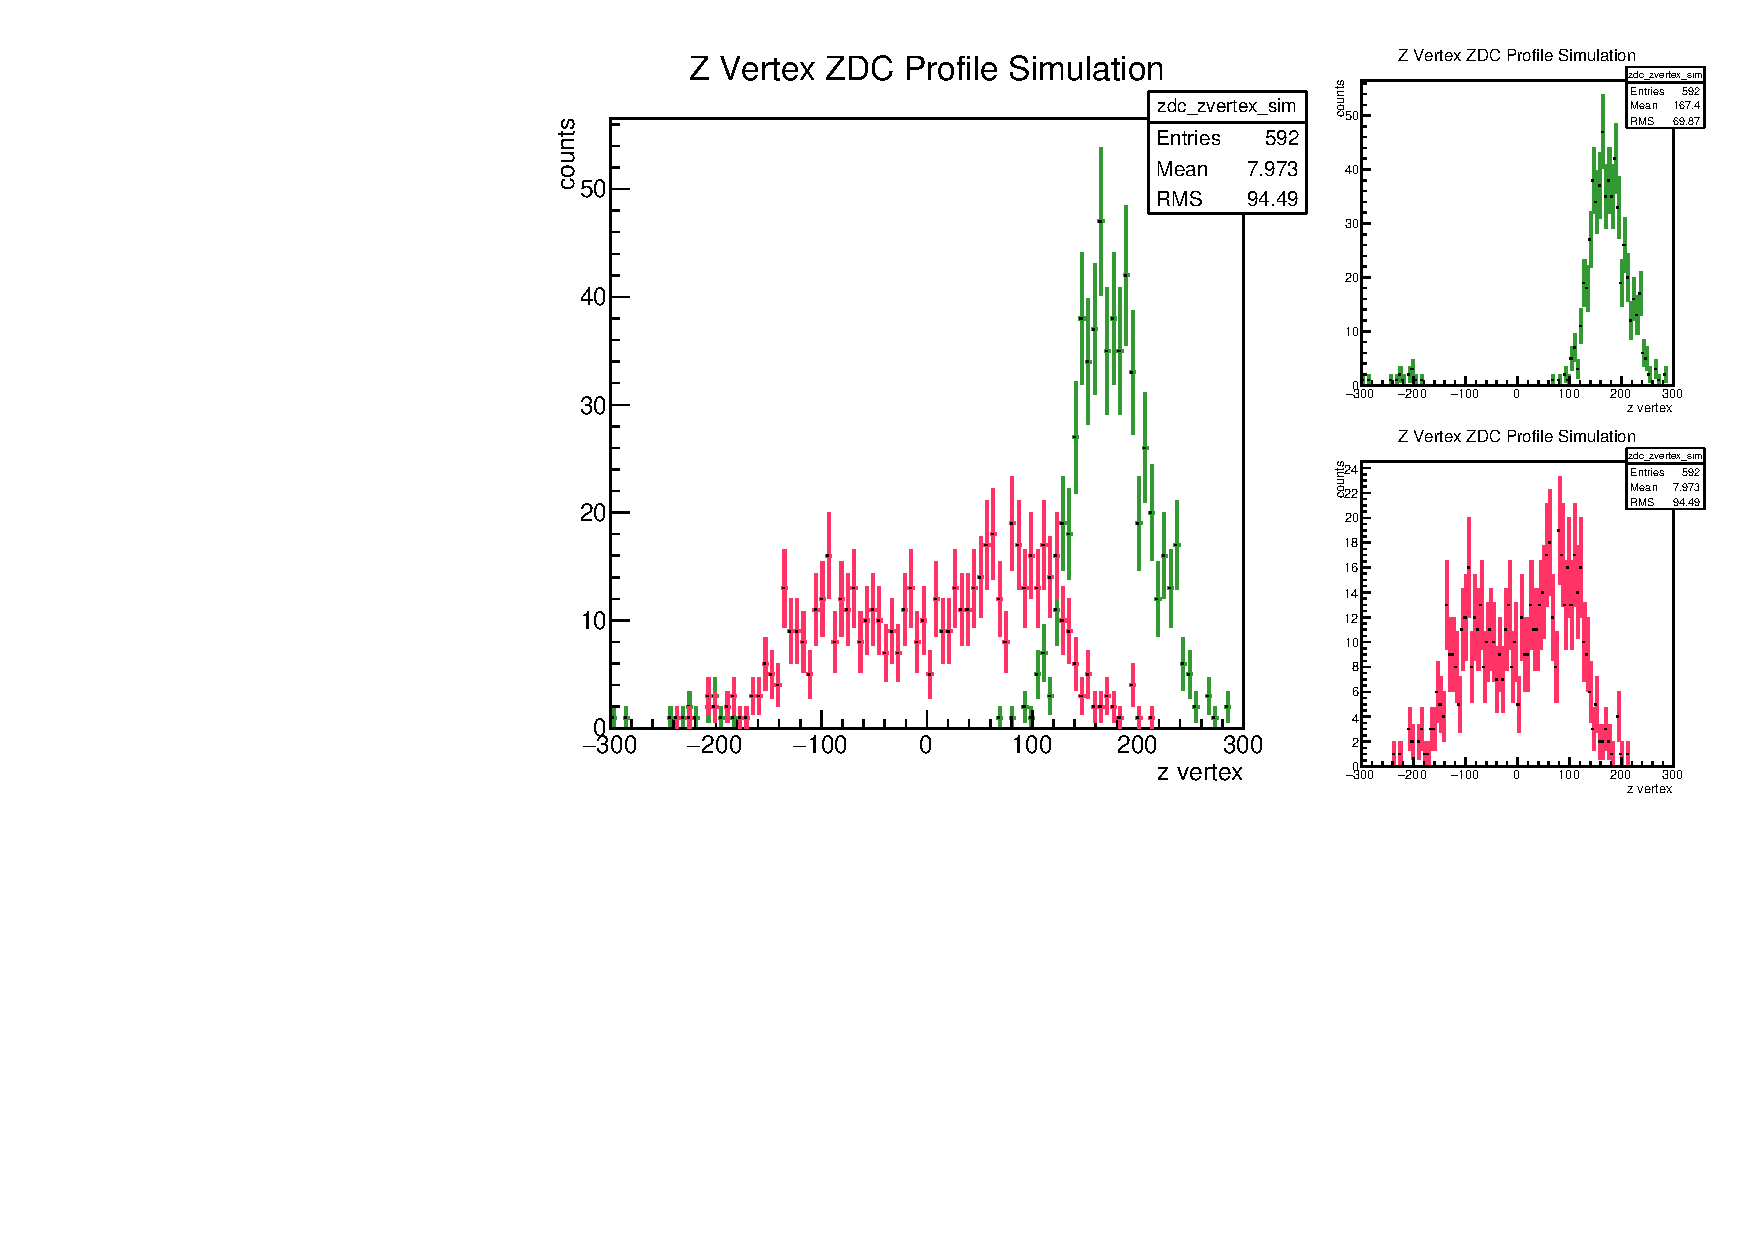
\includegraphics[width=\linewidth,height=\textheight,keepaspectratio]{../HourglassParameterSpace/figs/hsigma.pdf}
\end{frame}

\begin{frame}{Large and Small Z-bunch profile}
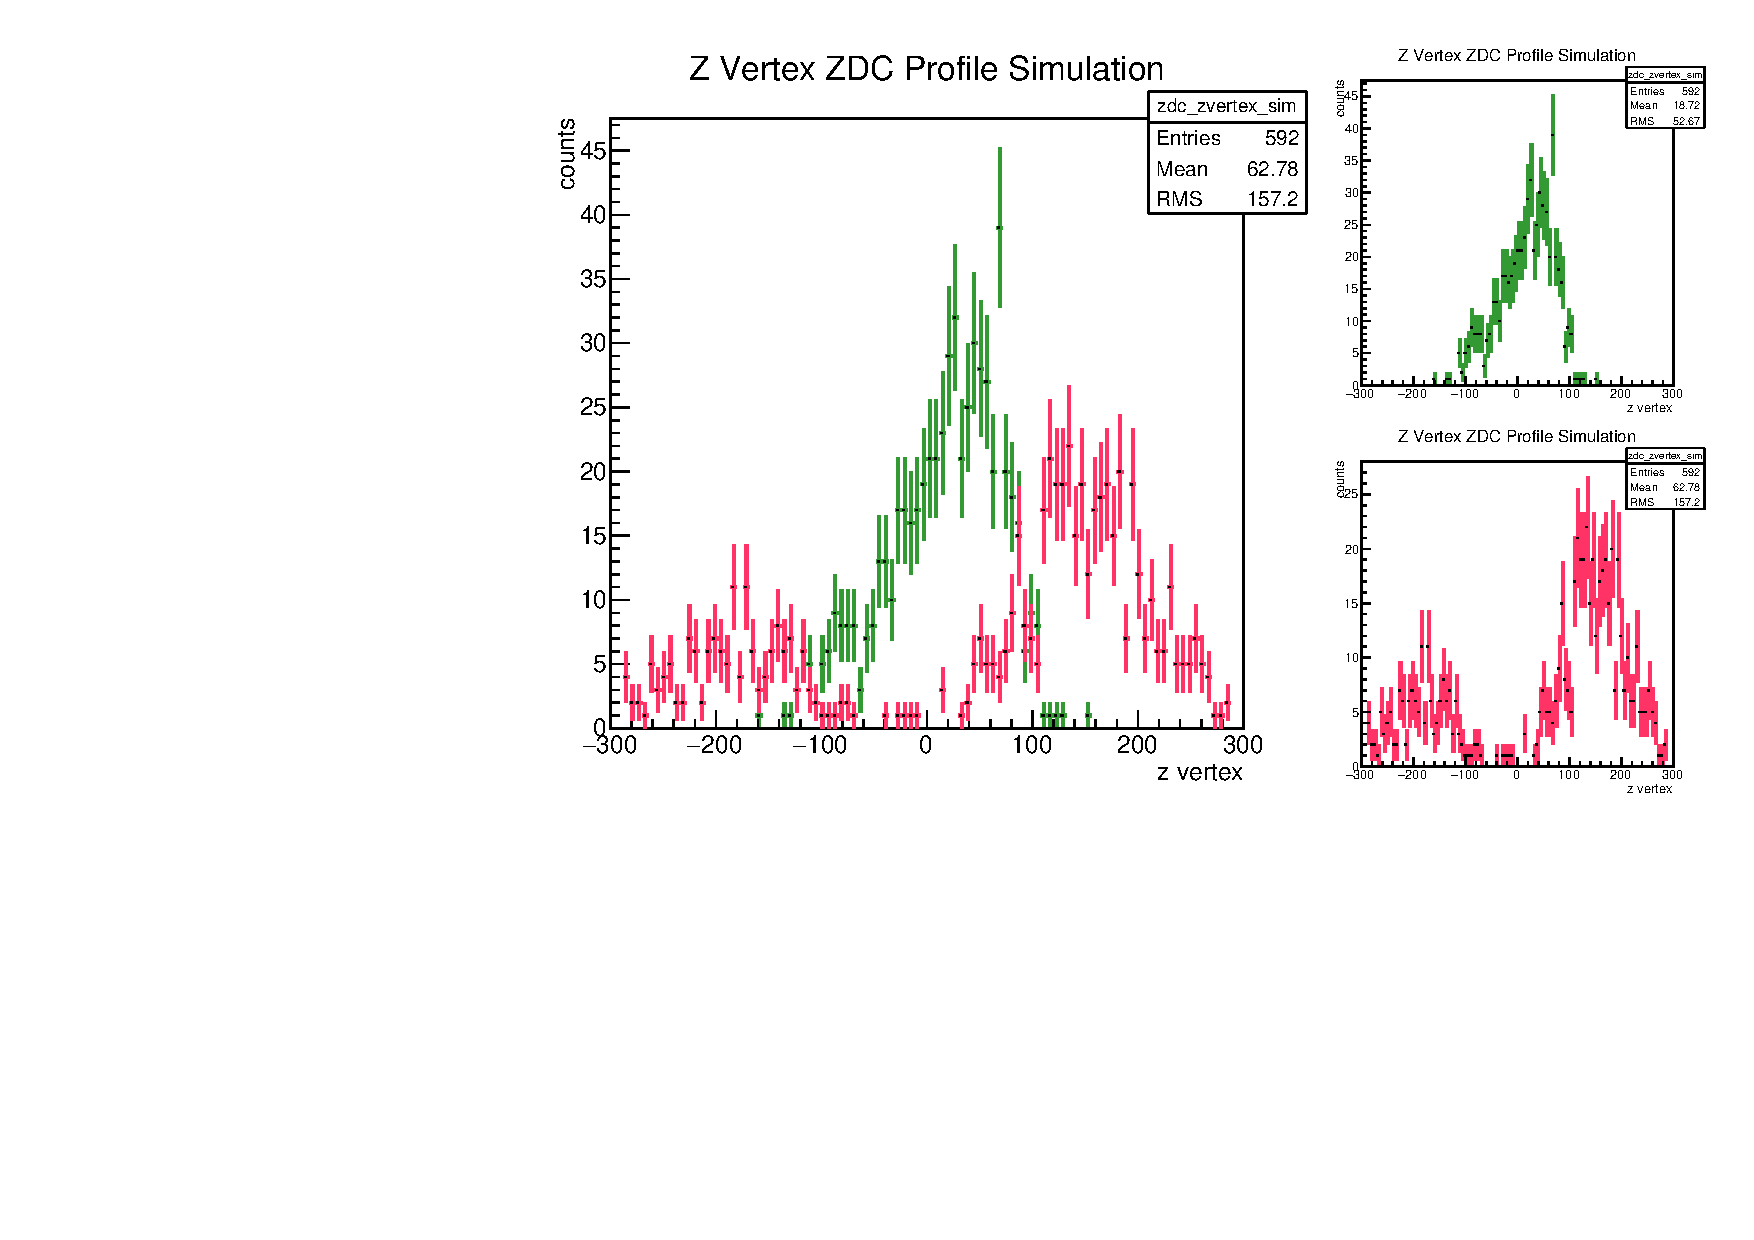
\includegraphics[width=\linewidth,height=\textheight,keepaspectratio]{../HourglassParameterSpace/figs/z_profile_scale.pdf}
\end{frame}

\begin{frame}{Large and Small $\sigma{y}$}
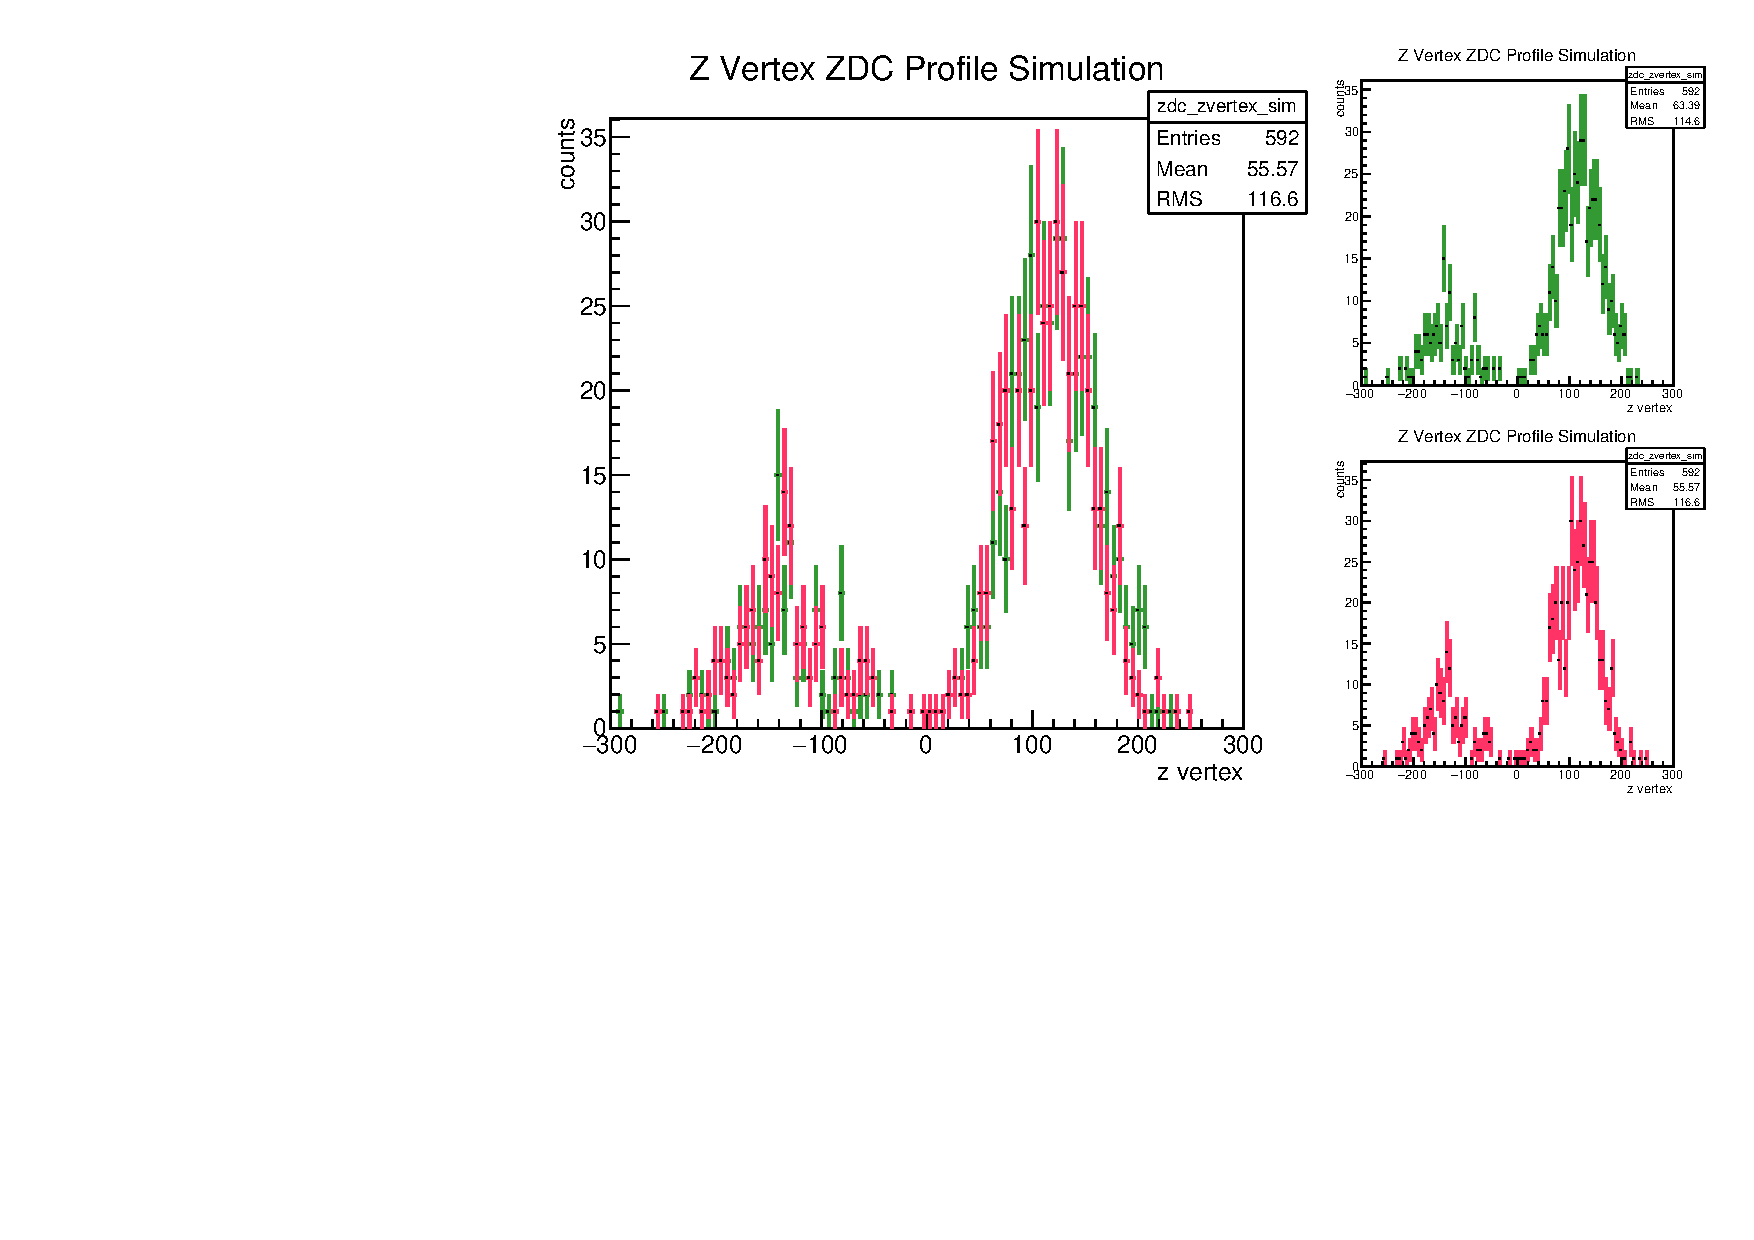
\includegraphics[width=\linewidth,height=\textheight,keepaspectratio]{../HourglassParameterSpace/figs/vsigma.pdf}
\end{frame}

\begin{frame}{Large and Small $\theta_{XZ}$ }
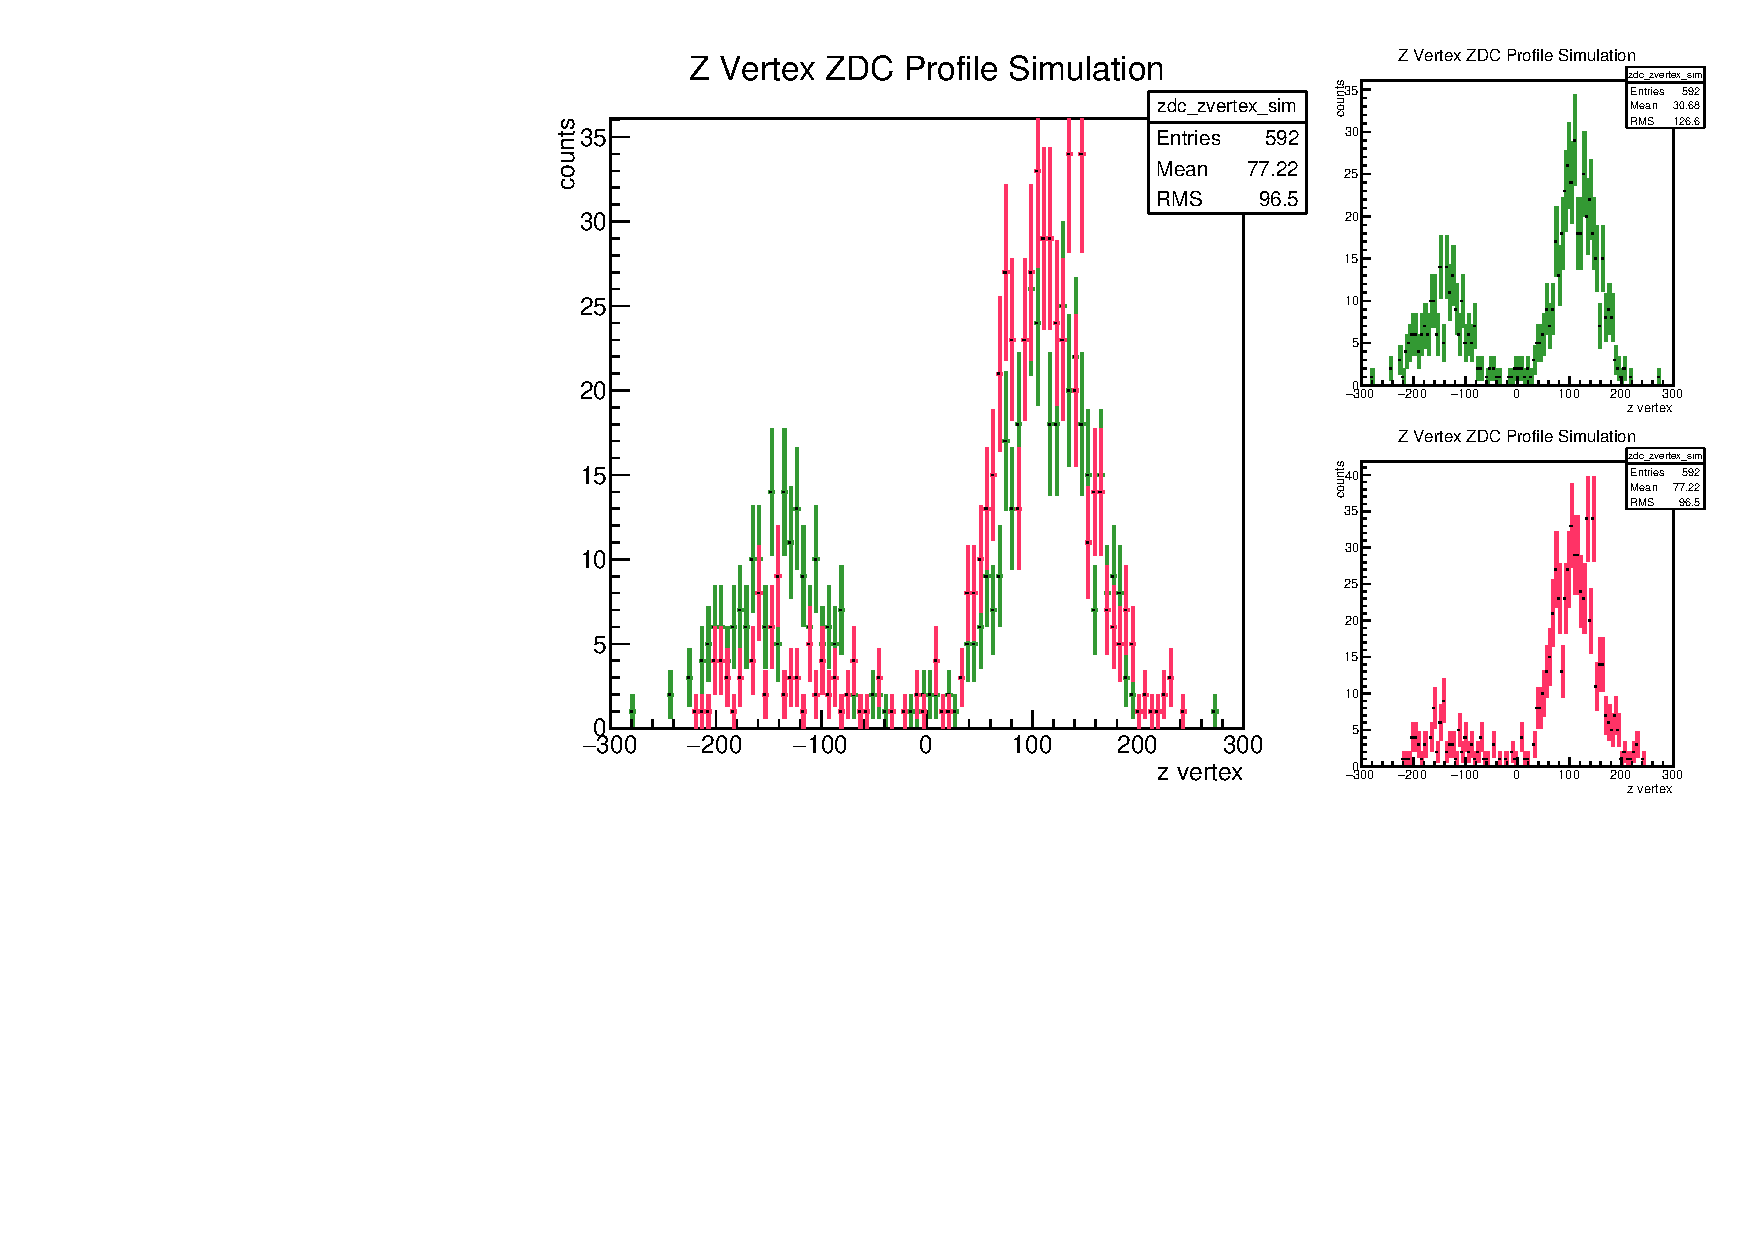
\includegraphics[width=\linewidth,height=\textheight,keepaspectratio]{../HourglassParameterSpace/figs/xz_angle.pdf}
\end{frame}

\begin{frame}{Exploring the Parameter Space}
Based on our exploration, we have confirmed/discovered that the following
parameters map to the following z-profile behavior:
\begin{itemize}
\item Z-Profile Scale $\rightarrow$ Stretching/Squeezing of distribution
\item $\theta_{XZ} \rightarrow$ Asymmetry in peak heights
\item Z-Profile $\rightarrow$ Individual Peak Widths
\item Beam Displacement / $\sigma{x,y} \rightarrow$ Peak Separation
\item ZDC yield (not shown) $\rightarrow$ Peak Scaling
\end{itemize}

Also note that scaling the beam widths OR changing the displacement will change
the total amount of overlapping beam. Note too that we cannot observe the
effects of vertical-beam width scaling or YZ crossing angle during a horizontal
beam displacement.
\end{frame}


\subsection{Modeling Bunch Z-Profile}
\begin{frame} {Modeling Z-Profile}
Here, I present my preliminary studies on the affect of z-profile of the bunches
in simulation on the final simulated z-vertex distribution.
\end{frame}


